%% LyX 2.2.3 created this file.  For more info, see http://www.lyx.org/.
%% Do not edit unless you really know what you are doing.
\documentclass[twoside,english]{article}
\usepackage[T1]{fontenc}
\usepackage[latin9]{inputenc}
\usepackage[a4paper]{geometry}
\geometry{verbose,lmargin=2cm,rmargin=2cm}
\usepackage{fancyhdr}
\pagestyle{fancy}
\setlength{\parindent}{0bp}
\usepackage{babel}
\usepackage{verbatim}
\usepackage{float}
\usepackage{amsmath}
\usepackage{graphicx}
\usepackage[unicode=true,
 bookmarks=true,bookmarksnumbered=false,bookmarksopen=false,
 breaklinks=false,pdfborder={0 0 1},backref=false,colorlinks=false]
 {hyperref}
\hypersetup{
 pdfauthor={Peter Lorenz}}

\makeatletter

%%%%%%%%%%%%%%%%%%%%%%%%%%%%%% LyX specific LaTeX commands.
\floatstyle{ruled}
\newfloat{algorithm}{tbp}{loa}
\providecommand{\algorithmname}{Algorithm}
\floatname{algorithm}{\protect\algorithmname}

%%%%%%%%%%%%%%%%%%%%%%%%%%%%%% User specified LaTeX commands.
\date{}

\usepackage{todonotes}
\bibliographystyle{plain}
\usepackage{fancyhdr}
\fancyhf{}% Clear header footer
\usepackage{listings}
    \usepackage{color}
    \definecolor{hellgelb}{rgb}{1,1,0.85}
    \definecolor{colKeys}{rgb}{0,0,1}
    \definecolor{colIdentifier}{rgb}{0,0,0}
    \definecolor{colComments}{rgb}{1,0,0}
    \definecolor{colString}{rgb}{0,0.5,0}
    \lstset{%
          language=Matlab,%
          float=hbp,%
          basicstyle=\footnotesize\ttfamily,%
          identifierstyle=\color{colIdentifier},%
          keywordstyle=\color{colKeys},%
          stringstyle=\color{colString},%
          commentstyle=\itshape\color{colComments},%
          columns=fixed,
          tabsize=4,%
          %frame=single,%
          extendedchars=true,%
          showspaces=false,%
          showstringspaces=false,%
          numbers=left,%
          numberstyle=\tiny\ttfamily,%
          numbersep=1em,%
          breaklines=true,%
          breakindent=10pt,
          breakautoindent=true,%
          captionpos=t,%
          xleftmargin=1em,%
          xrightmargin=\fboxsep%
    }

\makeatother

\usepackage{listings}
\renewcommand{\lstlistingname}{Listing}

\begin{document}

\lhead{LORENZ Peter, REICHEL Robert\hfill{} Assignment 3}

\section*{Octave 3.3}

Gegeben ist das System:

\begin{figure}[H]
\begin{centering}
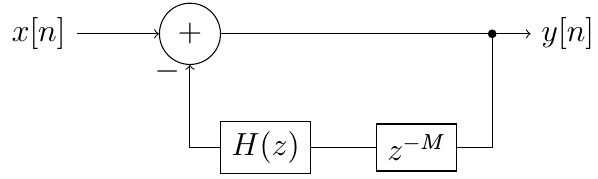
\includegraphics[scale=0.6]{system}
\par\end{centering}
\caption{System\label{fig:System}}
\end{figure}

Bei $H(z)$ spricht man von der z-Transformierte der Impulsantwort$h[n]$
und $z^{-M}$ ist die Verz�gerung um $M$ Samples.

\subsection*{a) Problem: Finde eine Differentialgleichung, die das System beschreibt
und bestimmen der $H_{1}(z)=\frac{Y(z)}{X(z)}$.}

Nach Umformung von der Abbildung \ref{fig:System} erhalten wir folgende
Differenzengleichung:

\[
y[n]=x[n]-h[n-m]
\]

Die zugeh�rige �bertragungsfunktion sieht folgenderma�en aus:

\begin{align*}
H_{1}(z) & =\frac{Y(z)}{X(z)}\\
Y(z) & =X(z)-H(z)z^{-M}Y(z)\\
Y(z)\left(H(z)z^{-M}+1\right) & =X(z)\\
H_{1}(z) & =\frac{Y(z)}{X(z)}=\frac{1}{1+H(z)z^{-M}}
\end{align*}

\subsection*{b) Problem: Eine Audiodatei einlesen und den Absolutbetrag plotten.}

\subsubsection*{Durchf�hrung in Matlab}

\begin{algorithm}[H]
\begin{lstlisting}
[x, fs] = audioread('Data/sample1.wav'); 
N = length(x); 
f = (0:(N-1))*fs/N;
xdft = fft(x); 
[~,index] = max(abs(xdft(1:length(x)/2+1)));
freq = 0:(fs/length(x)):fs/2;
\end{lstlisting}

\caption{Berechnung des Frequenzvektors\label{alg:Berechnung-des-Frequenzvektors}}
\end{algorithm}

\begin{figure}[H]
\begin{centering}
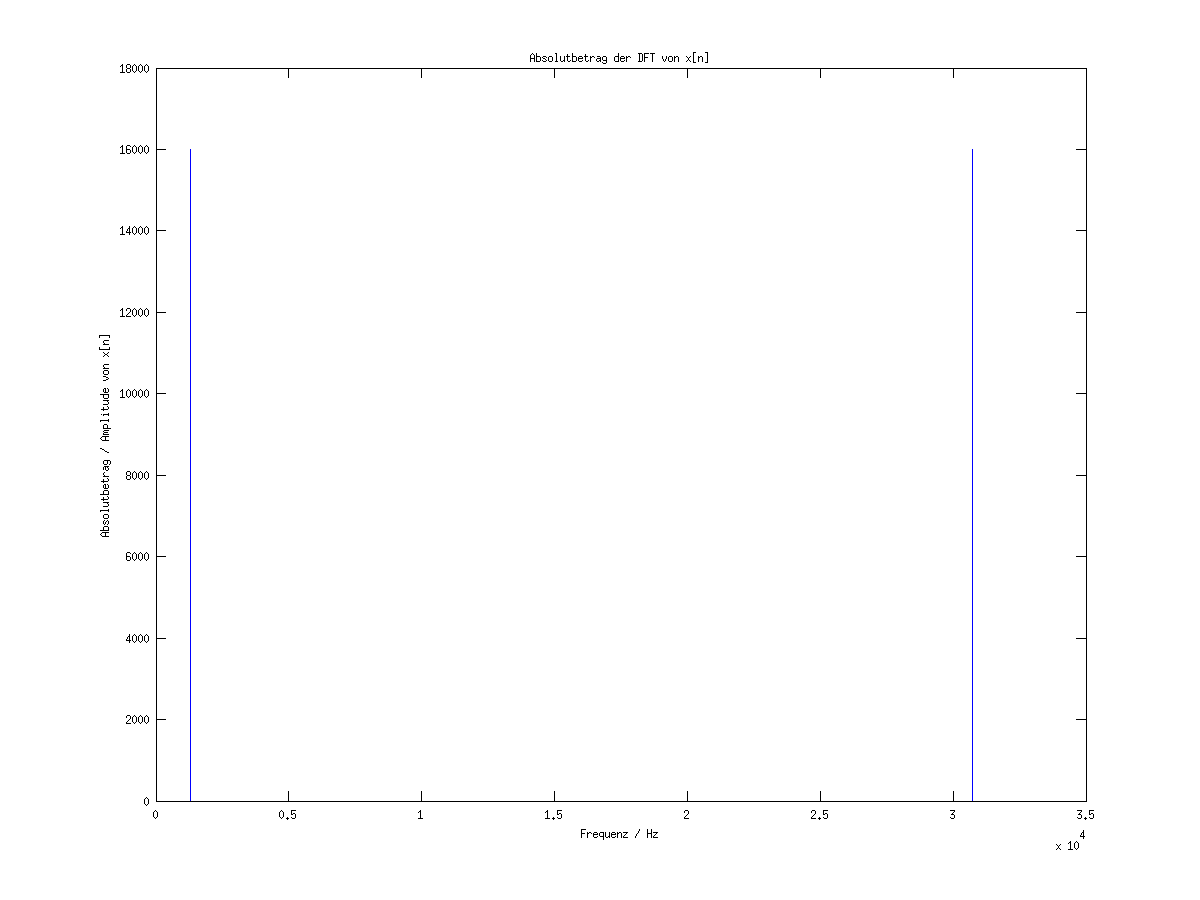
\includegraphics[scale=0.6]{img/33b}
\par\end{centering}
\caption{Grundfrequenz $f_{0}$ des zugrunde liegenden Signals - Absolutbetrag
von xdft}
\end{figure}

\subsection*{c)Problem: Plot der ersten Periode von $x$}

In Punkt a wurde die Grundfrequenz $f_{0}$ ermittelt. Mit dieser
kann die Periodendauer $T_{0}$ ermittelt werden:

\[
T_{0}=\frac{1}{f_{0}}
\]

Jetzt wissen wir nur die Periodendauer $T_{0}$, aber nicht wieviele
Samples dabei sein sollen. Dazu muss die Samplefrequenz mit der gr��ten
Amplitude dividiert werden. 

\[
samples=\frac{f_{s}}{f[index]}=25
\]

\subsubsection*{Durchf�hrung in Matlab}

\begin{algorithm}[H]
\begin{lstlisting}
T_0 = 1/f(index); 
cnt_samples = fs / f(index);
fig = figure(201); 
y_axis = (0:1/fs:T_0); 
plot(y_axis(1:cnt_samples), x(1:cnt_samples)); 
title('Signal x1'); 
ylabel('x1[n]'); xlabel('n in s');
\end{lstlisting}

\caption{Berechnung des Frequenzvektors}
\end{algorithm}

Wie in der Problemstellung erkl�rt wird die Periodendauer ben�tigt,
jedoch die Variable \emph{index} wurde schon fr�her ermittelt, siehe
Listing \ref{alg:Berechnung-des-Frequenzvektors}.

\begin{figure}[H]
\begin{centering}
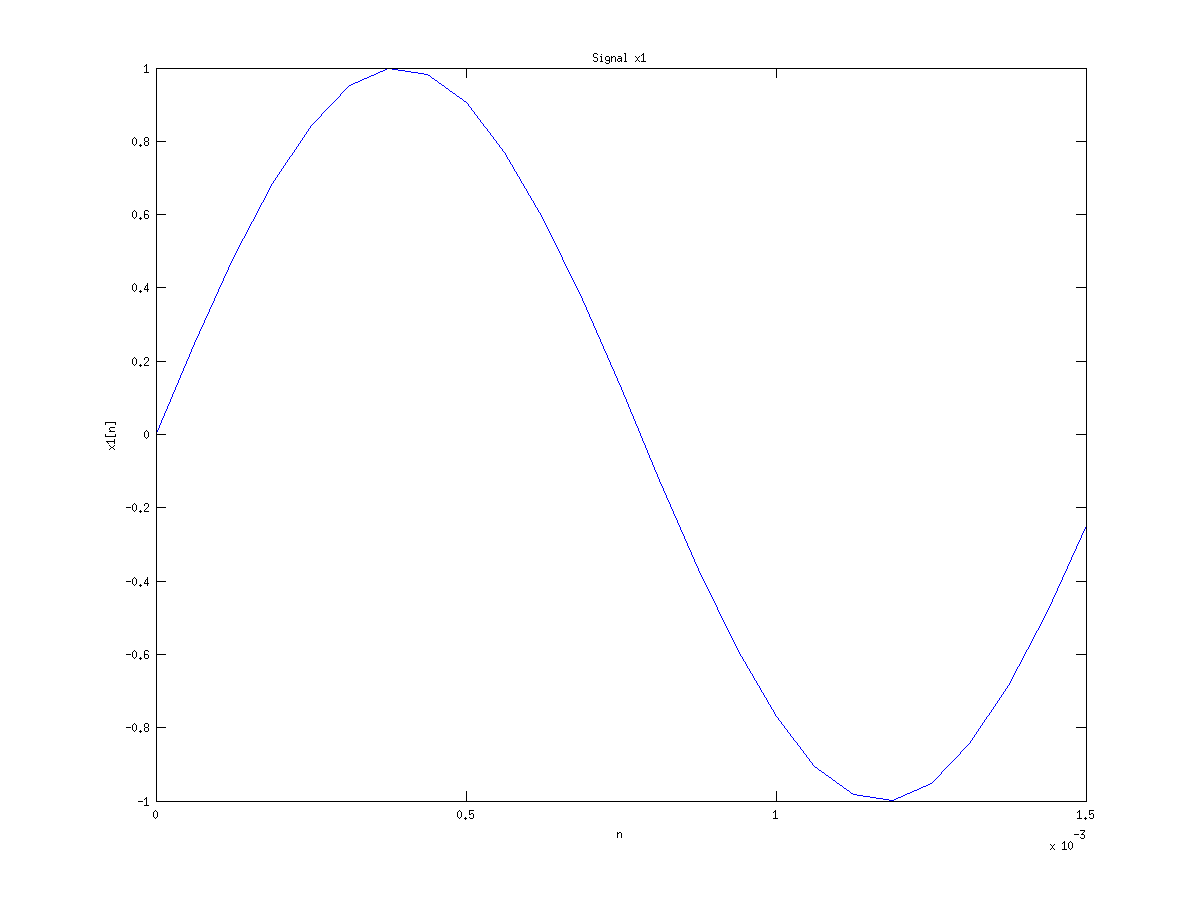
\includegraphics[scale=0.6]{img/33c}
\par\end{centering}
\caption{1 Periodendauer des Signals $x[n]$}
\end{figure}

\subsection*{d) Welchen Wert muss $\alpha$ annehmen, dass $H_{1}(z)$ stabil
ist?}

Wir wissen aus vorherigen Berechnungen, dass
\begin{itemize}
\item $M=T_{0}\cdot fs=25$
\item $H(z)=\alpha$
\end{itemize}
Was muss $\alpha$ erf�llen, damit $H_{1}(z)$ stabil ist? 

Wir wissen, dass $H_{1}(z)=\frac{1}{1+z^{\text{-}M}\alpha}$.

Damit ein System stabil ist, muss der Einheitskreis im ROC sein. Das
bedeutet, dass alle Pole im Einheitskreis liegen m�ssen. Der Pol von
$H_{1}(z)$ errechnet sich durch 
\[
1+z^{-M}\cdot\alpha=0
\]

Wir wissen dass Pole die From von $z-z_{0}$ haben und k�nnen die
obrigen Term umformen:

\[
z^{-M}+\frac{1}{\alpha}=0
\]

Nun muss $\alpha$ so gew�hlt werden, dass der Bruch $\frac{1}{\alpha}<1$
bleibt, damit die Pole im Einheitskreis bleiben. Daraus folgt, dass
$\alpha>1\vee\alpha<-1$ sein muss. 

\subsection*{e) Problem: KS-algorithm}

\subsubsection*{Durchf�hrung in Matlab}

\begin{figure}[H]
\begin{centering}
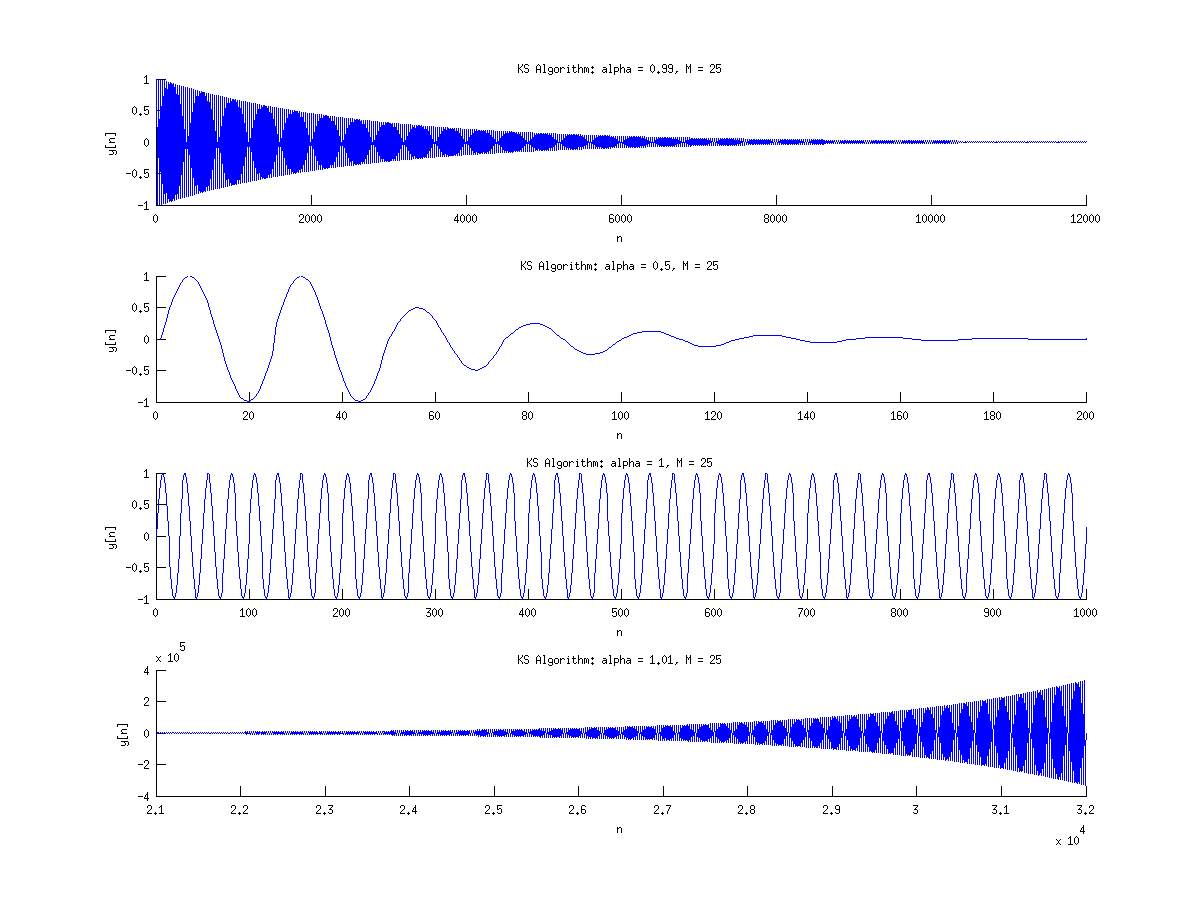
\includegraphics[scale=0.6]{img/33g}
\par\end{centering}
\caption{KS Algorithmus mit $\alpha=\{0.99,0.5,1.00,1.01\}$}
\end{figure}

\subsection*{f) Problem: }

\subsubsection*{Durchf�hrung in Matlab}

\begin{figure}[H]
\begin{centering}
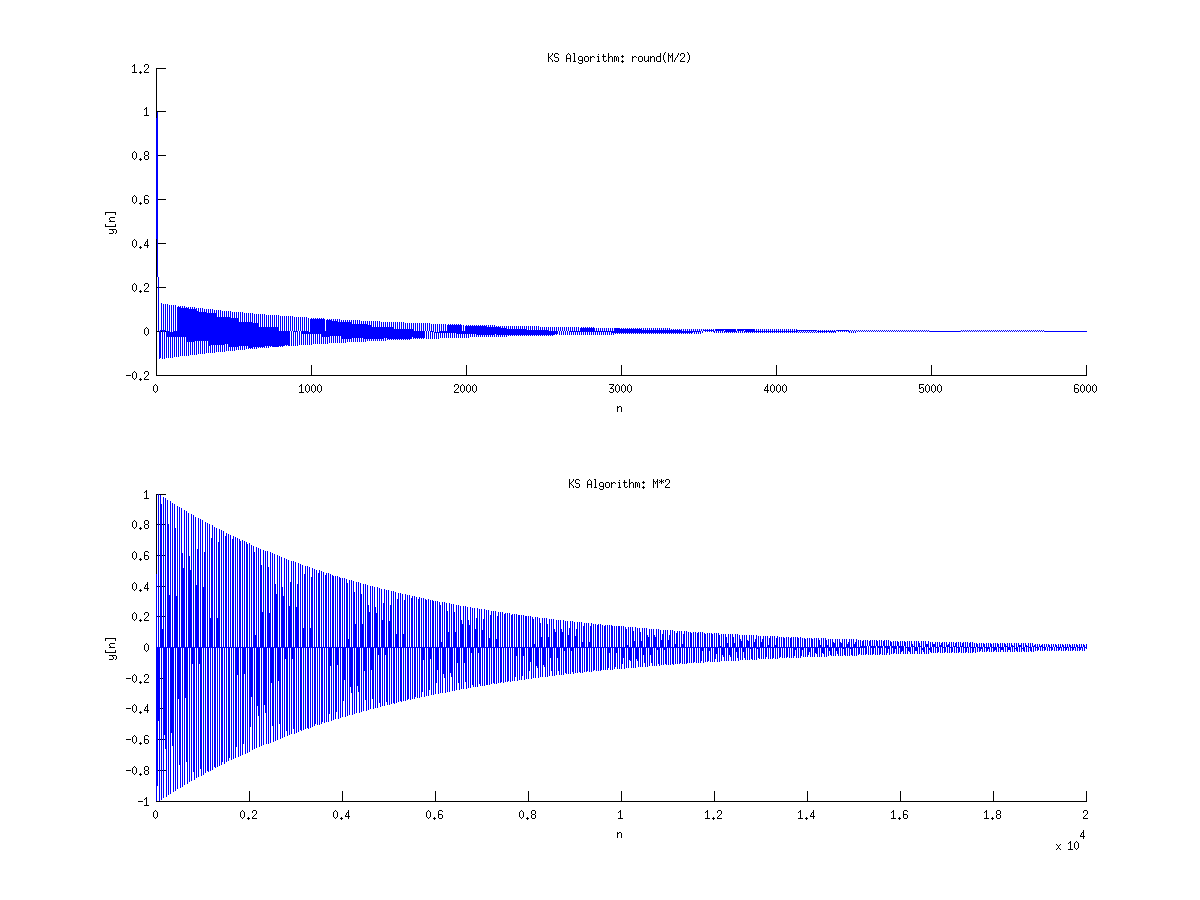
\includegraphics[scale=0.6]{img/33f}
\par\end{centering}
\caption{}
\end{figure}

\subsection*{g) Problem: }

\subsubsection*{Durchf�hrung in Matlab}

\begin{figure}[H]
\begin{centering}
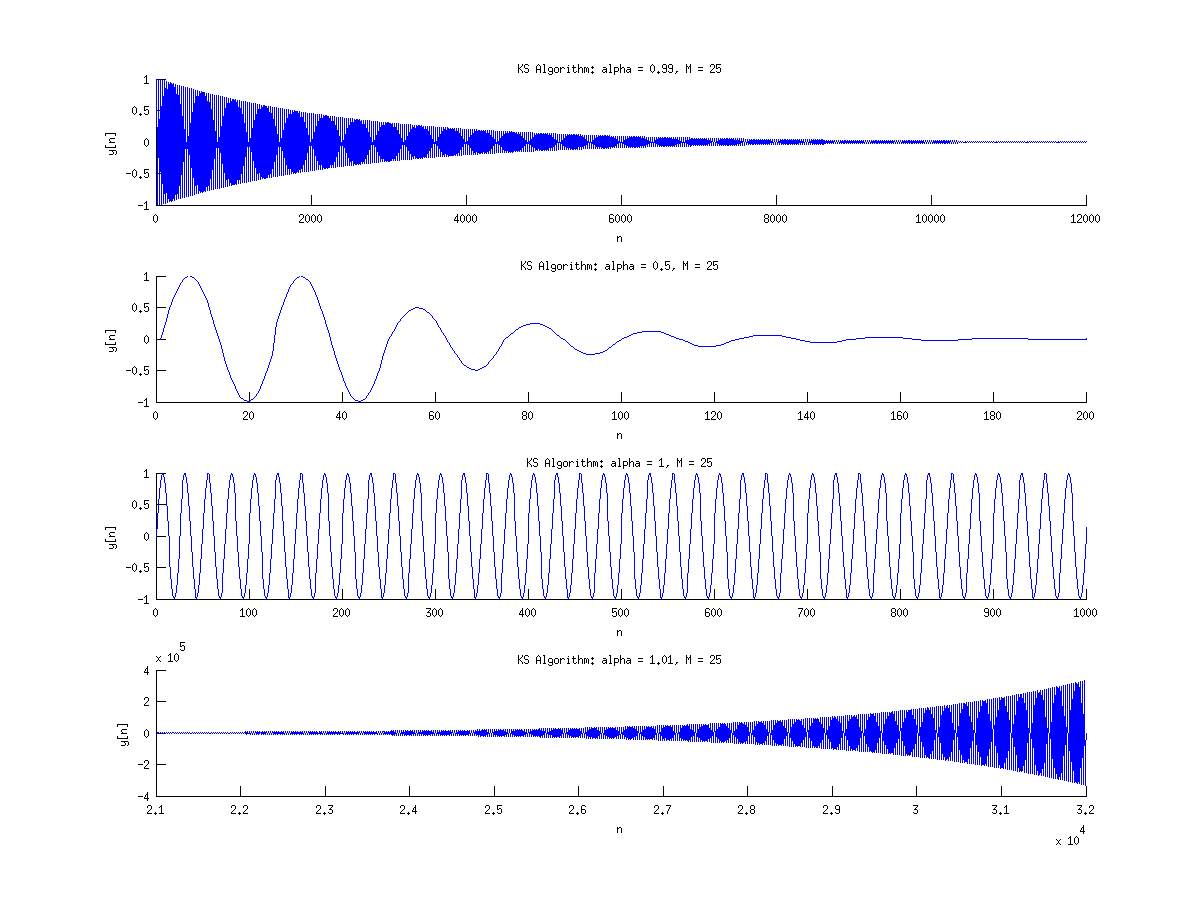
\includegraphics[scale=0.6]{img/33g}
\par\end{centering}
\caption{KS Algorithmus mit $\alpha=\{0.99,0.5,1.00,1.01\}$}
\end{figure}

\subsection*{h) {[}Bonus{]} Problem:}

\subsubsection*{Durchf�hrung in Matlab}

\begin{figure}[H]
\begin{centering}
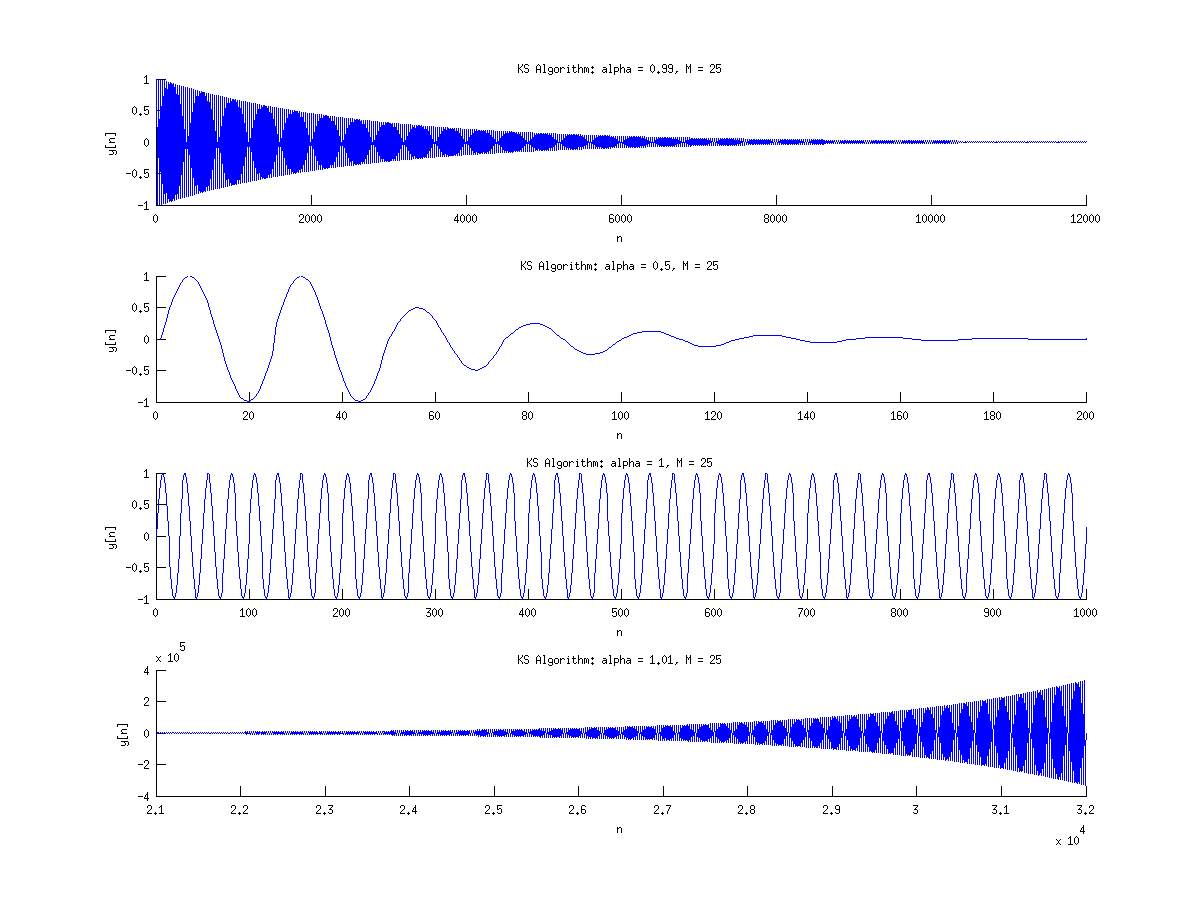
\includegraphics[scale=0.6]{img/33g}
\par\end{centering}
\caption{}
\end{figure}

\subsection*{i) {[}Bonus{]} Problem: }

\subsubsection*{Durchf�hrung in Matlab}

\begin{algorithm}[H]
\begin{lstlisting}
X = load('Data/Measurement.mat');
b = cell2mat(struct2cell(X)); 
br = reshape(b, [1,2048]); 
X2 = fliplr(br);
X = [br X2]; 
x = ifftreal(X); 
f = (0:length(X)-1)*100/length(X);  
phase = radtodeg(angle(X));
\end{lstlisting}

\caption{Laden und Vorbereiten der Messdaten}
\end{algorithm}

Der Algorithmus f�r ifftreal(X) hat vom Formelzettel Seite 2 die Gleichung
$X[k]=\sum_{n=0}^{N-1}x[n]e^{-j\frac{2\pi}{N}nk}$ implementiert.

\begin{algorithm}[H]
\begin{lstlisting}
function [ x ] = ifftreal( X ) 
   N = length(X);     
   tmp = zeros(N,N);     
   for n = 0:N-1         
      for k = 0:N-1             
          tmp(k+1,n+1) = exp(1j*2*pi*n*k/N);         
      end     
   end
   x = X * (1/N .* tmp); 
end
\end{lstlisting}

\caption{ifftreal(X)}
\end{algorithm}

\begin{figure}[H]
\begin{centering}
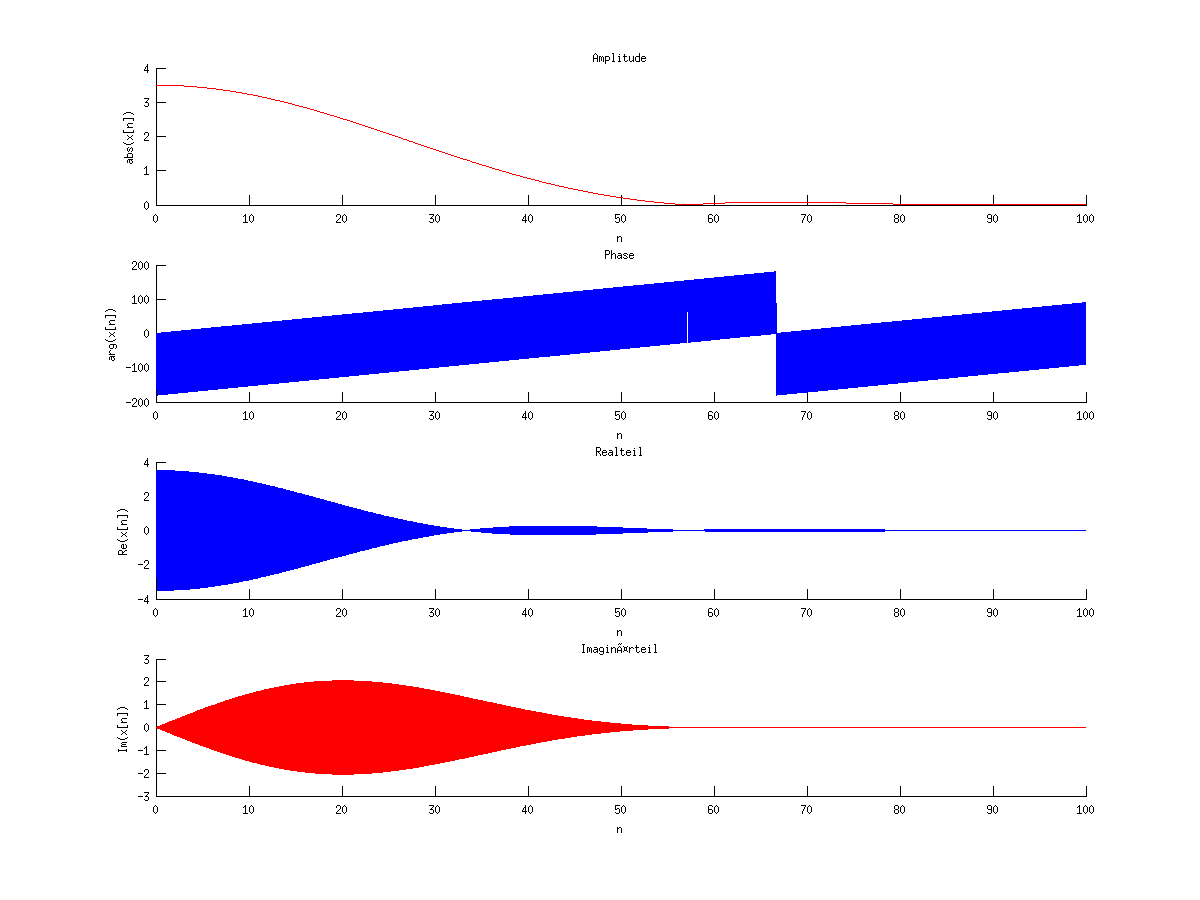
\includegraphics[scale=0.6]{img/33i}
\par\end{centering}
\caption{Amplitute, Phase, Realteil und Imagin�rteil der $N_{FFT}$-Punkte
langen DFT von $x[n]$}
\end{figure}

Wie verhalten sich Realteil und Imagin�rteil (bzw. Amplitute und Phase)?
\begin{comment}
Generieren Sie eine Darstellung des Zeitsignals x{[}n{]}.
\end{comment}

\end{document}
